\documentclass{beamer}
\usepackage[latin1]{inputenc}
\usepackage{comment}
%\usepackage[3D]{movie15}
\usetheme{Warsaw}
\usecolortheme{beaver}
\usefonttheme{structuresmallcapsserif}

\setbeamertemplate{section page}
{
     \tableofcontents[currentsection,hideothersubsections]
}
\setbeamertemplate{subsection page}
{
     \tableofcontents[sectionstyle=show/shaded,subsectionstyle=show/shaded/hide]
}

%\AtBeginSection{\frame{\sectionpage}}
%\AtBeginSubsection{\frame{\subsectionpage}}

\DeclareMathOperator*{\argmin}{arg\,min}
\DeclareMathOperator{\diag}{diag}

\title{Pattern Recognition}
\author{Bertrand Thirion and John Ashburner}
%\institute[j.ashburner@ucl.ac.uk]{Wellcome Trust Centre for Neuroimaging,\\
%UCL Institute of Neurology,\\
%12 Queen Square,\\
%London WC1N 3BG,\\
%UK.}
\date{}
\begin{document}

\begin{frame}
\titlepage
\end{frame}

\section{Introduction}
    \subsection{Definitions}
\begin{frame}
\frametitle{}
\hspace*{-1.2cm}
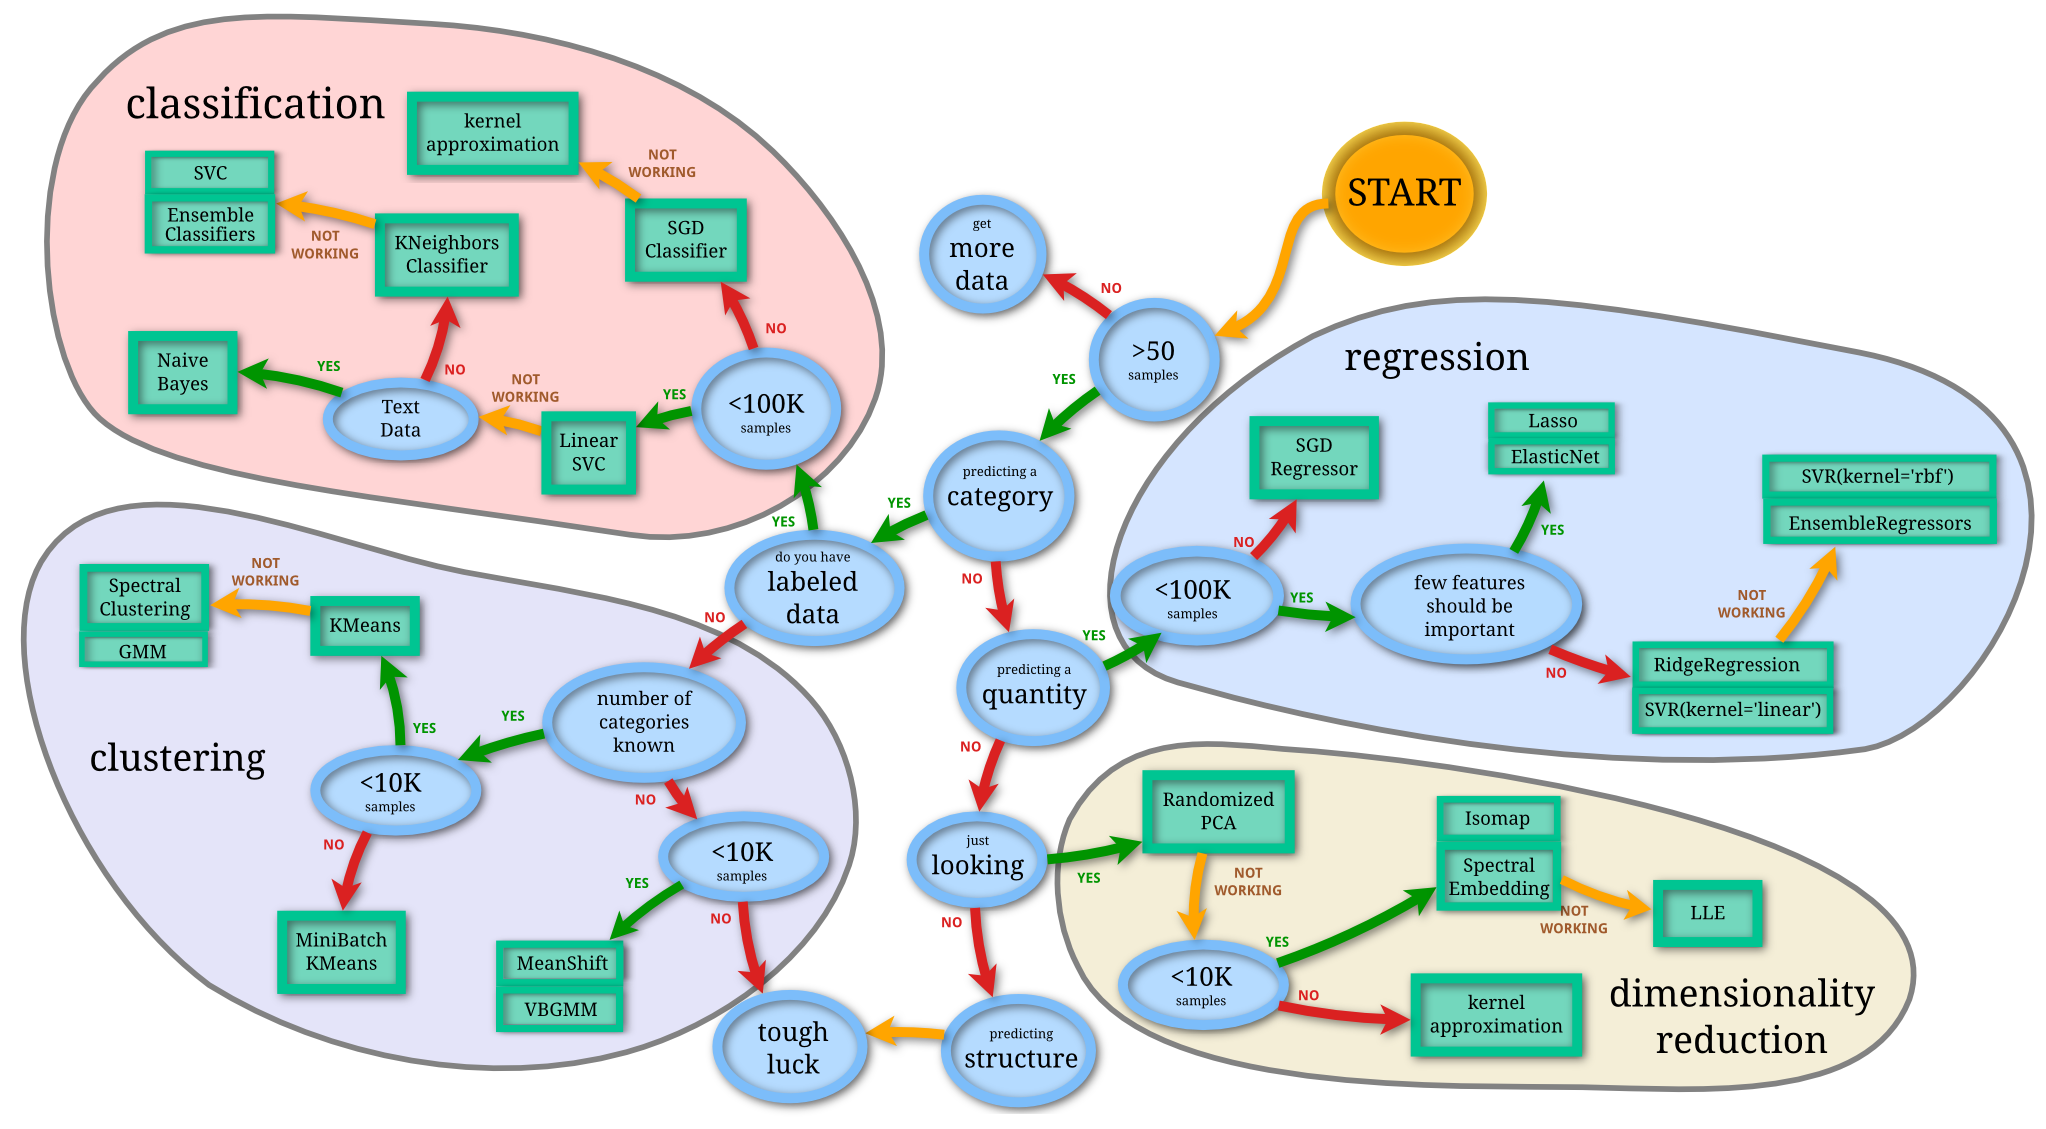
\includegraphics[width=1.2\textwidth]{sklearn_material/overview.png}
% Note: need some adaptation. Should not be sklearn specific
% useful to clarify the different branches of ML
% 
\end{frame}


\begin{frame}
\frametitle{Some key concepts}



\textbf{supervised learning}: The data comes with additional
attributes that we want to predict $\Longrightarrow$
classification and regression.\\
\vspace{1cm}

\textbf{unsupervised learning}: No target values. 
\begin{itemize}
\item
Discover groups of similar examples within the data (clustering).
\item
Determine the distribution of data within the input space (density estimation).
\item
Project the data down to two or three dimensions for visualization.
\end{itemize}

\end{frame}




    \subsection{Classification and Regression}                               \begin{frame}
\frametitle{General supervised learning setting}
We have a training dataset of $n$ observations, each consisting of an input ${\bf x}_i$ and a target $y_i$.\par
Each input, ${\bf x}_i$, consists of a vector of $p$ features.
\begin{align*}
\mathcal{D} = \{({\bf x}_i,y_i) | i=1,..,n\}
\end{align*}

The aim is to predict the target for a new input ${\bf x}_*$.
\end{frame}

\begin{frame}
\frametitle{Classification}
\begin{columns}
\column{0.4\textwidth}
Targets (${\bf y}$) are categorical labels.\par
Train with $\mathcal{D}$ and use result to make best guess of $y_*$ given ${\bf x}_*$.
\column{0.6\textwidth}
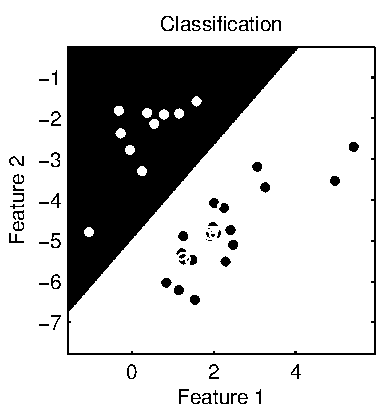
\includegraphics[width=\textwidth]{simple_classification}
\end{columns}
\end{frame}

\begin{frame}
\frametitle{Probabilistic classification}
\begin{columns}
\column{0.4\textwidth}
Targets (${\bf y}$) are categorical labels.\par
Train with $\mathcal{D}$ and compute $P(y_*=k | {\bf x}_*, \mathcal{D})$.
\column{0.6\textwidth}
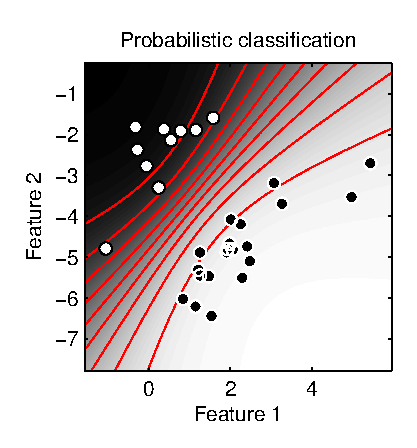
\includegraphics[width=\textwidth]{probabilistic_classification}
\end{columns}
\end{frame}

\begin{frame}
\frametitle{Regression}
\begin{columns}
\column{0.4\textwidth}
Targets (${\bf y}$) are continuous real variables.\par
Train with $\mathcal{D}$ and compute $p(y_* | {\bf x}_*, \mathcal{D})$.
\column{0.6\textwidth}
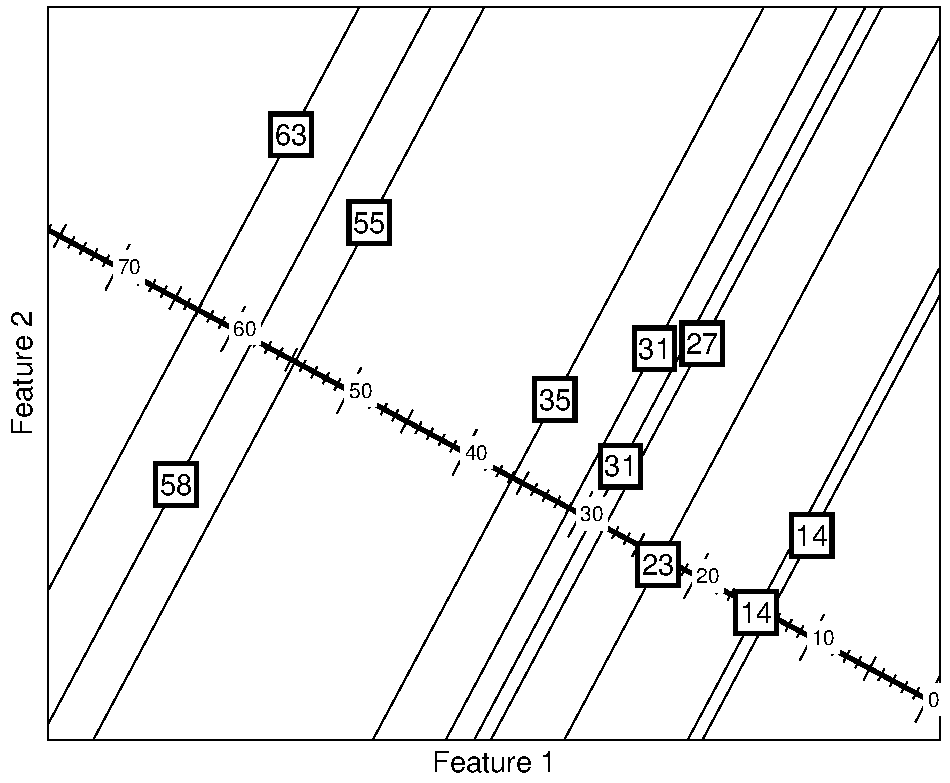
\includegraphics[width=\textwidth]{regression}
\end{columns}
\end{frame}

\begin{frame}
\frametitle{Many other settings}
\begin{itemize}
\item {\bf Multi-class classification} when there are more than two possible categories.
\item {\bf Ordinal regression} for classification when there is some ordering of the categories.\par
\begin{tiny}
Chu, Wei, and Zoubin Ghahramani. ``Gaussian processes for ordinal regression.'' In Journal of Machine Learning Research, pp. 1019-1041. 2005.\par
\end{tiny}
\item {\bf Multi-task learning} when there are multiple targets to predict, which may be related.
\item etc
\end{itemize}
\end{frame}

\begin{frame}
\frametitle{Multi-Class classification}

\begin{columns}
\column{.5\textwidth}
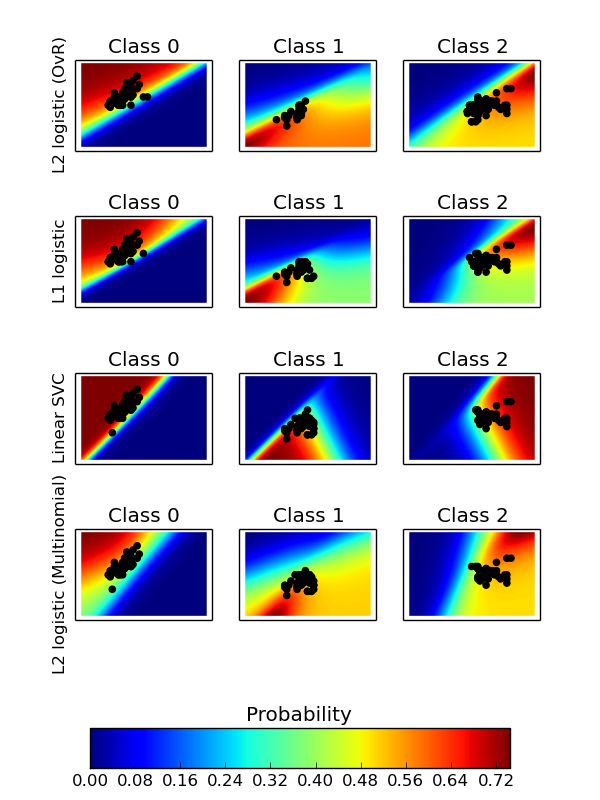
\includegraphics[width=\textwidth]{sklearn_material/plot_classification_probability_001.png}
\column{.6\textwidth}
\begin{itemize}
\item {\bf Multinomial Logistic regression} Theoretically optimal. Expensive optimization. 
\item {\bf One-versus-all classification} [SVMs] Among several
  models, pick the one with highest score. \\$\Longrightarrow$
  recommended
\item {\bf One-versus-one classification} Vote across each pair of
  class. Expensive, not optimal.
\end{itemize}
\end{columns}
\end{frame}


    \subsection{Curse of Dimensionality}                                     \begin{frame}
\frametitle{Curse of dimensionality}
\begin{center}
{\Huge Large $p$, small $n$.\par}
\end{center}
\end{frame}

\begin{frame}
\frametitle{Nearest-neighbour classification}
\begin{columns}[c]
\column{0.7\textwidth}
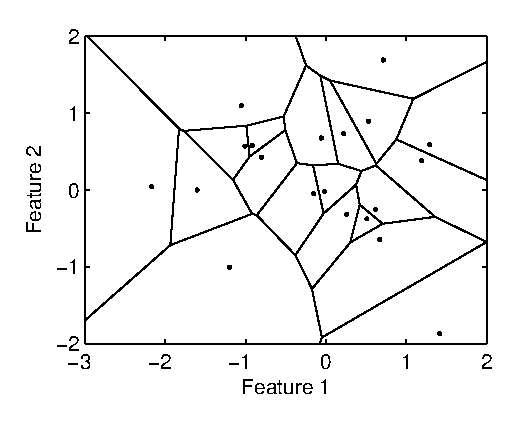
\includegraphics[width=\textwidth]{voronoi}
\column{0.3\textwidth}
\begin{itemize}
\item Not nice smooth separations.
\item Lots of sharp corners.
\item May be improved with \emph{K-nearest neighbours}.
\end{itemize}
\end{columns}
\end{frame}

\begin{frame}
\frametitle{Rule-based approaches}
\begin{columns}[c]
\column{0.7\textwidth}
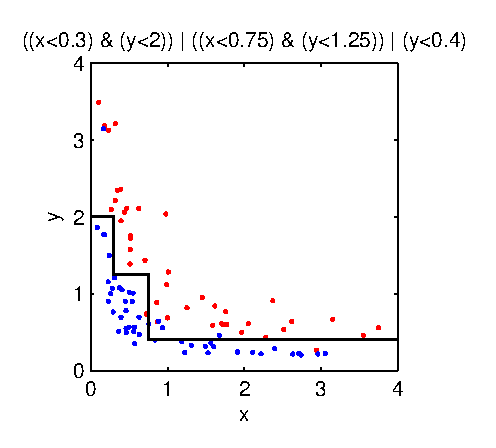
\includegraphics[width=\textwidth]{rule_based}
\column{0.3\textwidth}
\begin{itemize}
\item Not nice smooth separations.
\item Lots of sharp corners.
\end{itemize}
\end{columns}
\end{frame}


\begin{frame}
\frametitle{Corners matter in high-dimensions}
\begin{columns}[c]
\column{0.4\textwidth}
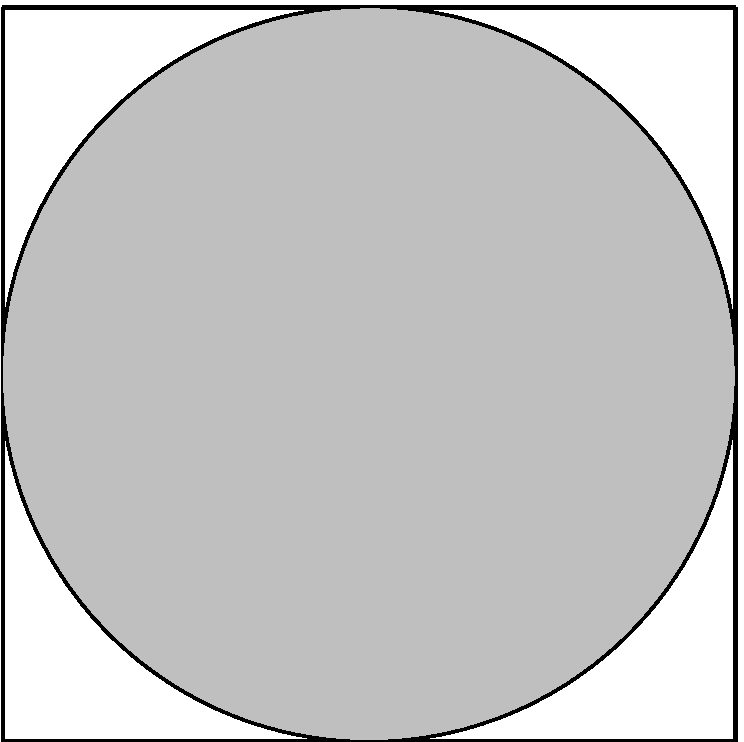
\includegraphics[width=\textwidth]{circle}
\column{0.6\textwidth}
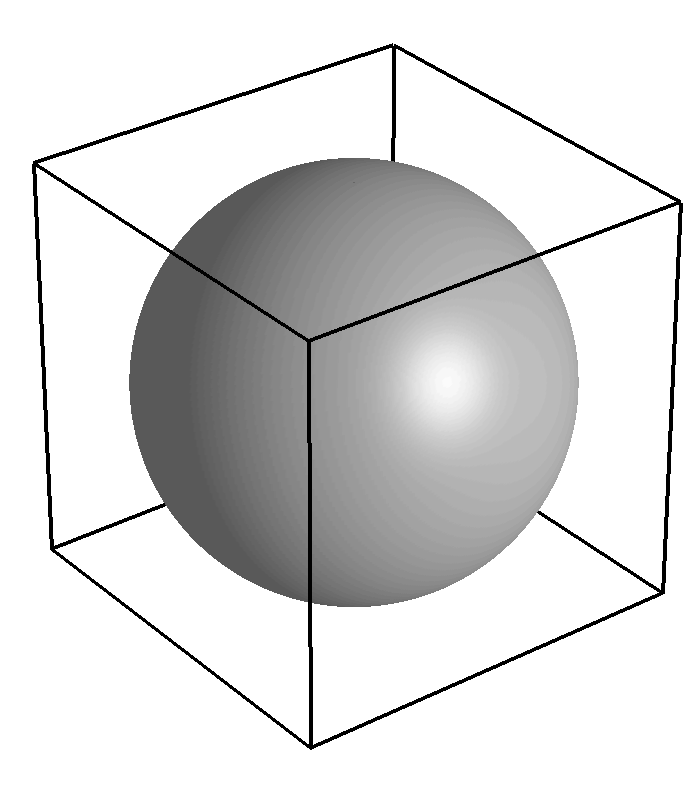
\includegraphics[width=\textwidth]{sphere}
\end{columns}
\end{frame}

\begin{frame}
\frametitle{Corners matter in high-dimensions}
\begin{columns}[c]
\column{0.2\textwidth}
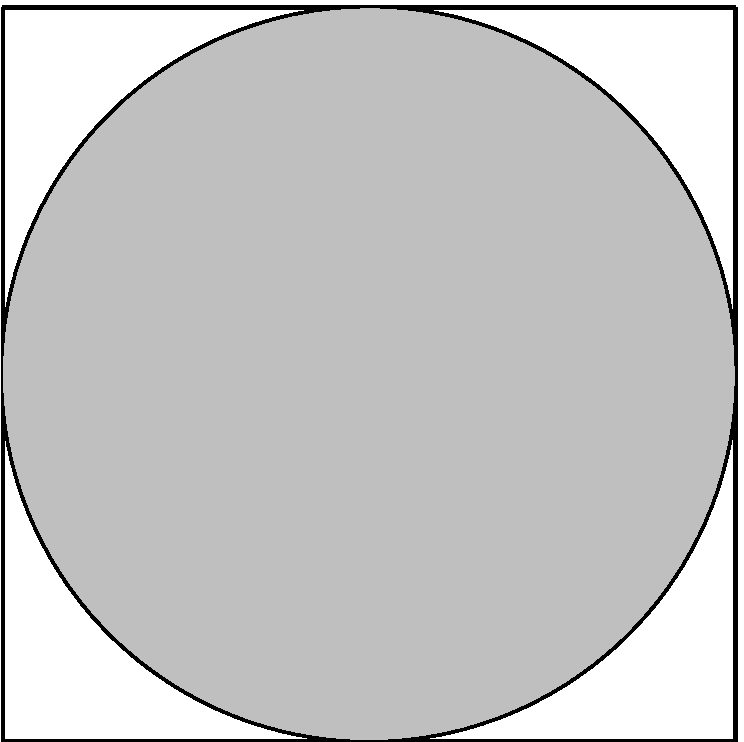
\includegraphics[width=.8\textwidth]{circle}

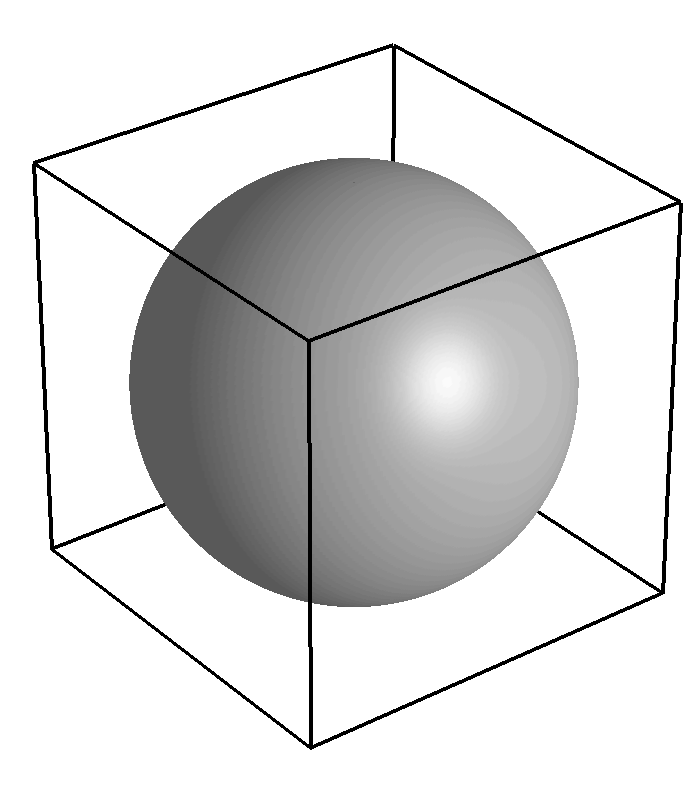
\includegraphics[width=\textwidth]{sphere}
\column{0.8\textwidth}
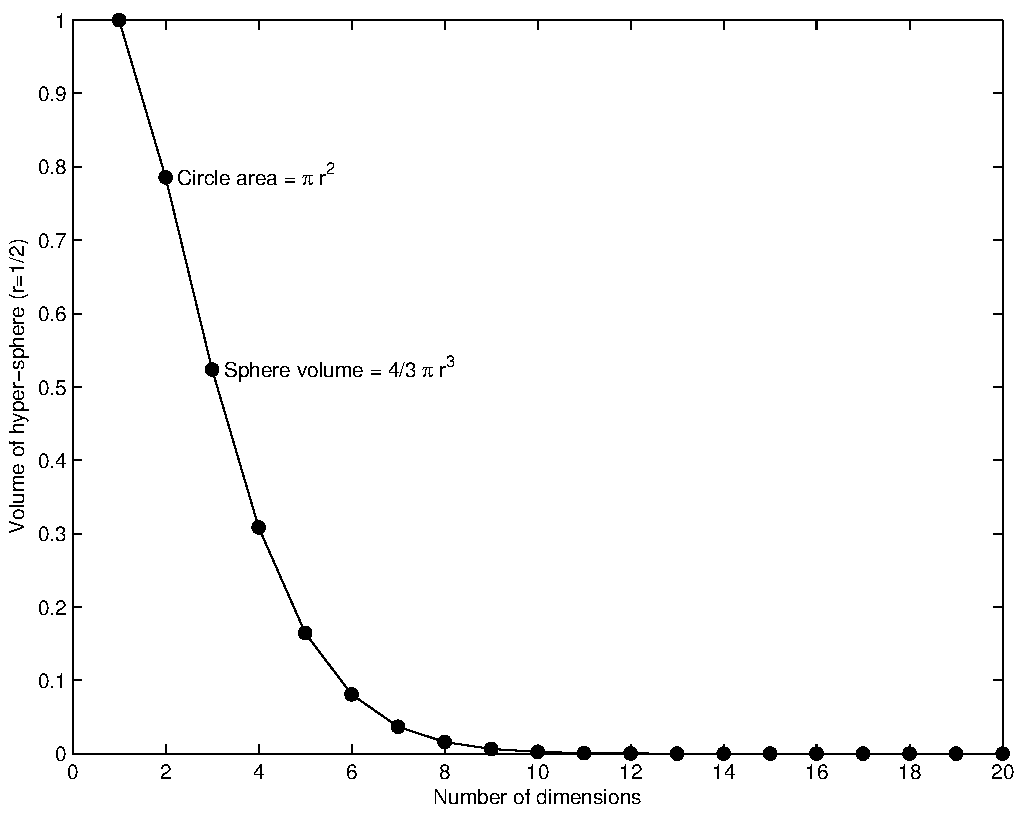
\includegraphics[width=\textwidth]{corners}
\end{columns}
\end{frame}


\section{Generalization of learned models across datasets}
    \subsection{Cross-Validation}                                            
\begin{frame}
\frametitle{Occam's razor}
\begin{quote}
``Everything should be kept as simple as possible, but no simpler.''
\par \rightline{\tiny{\rm --- Einstein (allegedly)}}
\end{quote}
\vspace{0.25cm}
\begin{itemize}
\item Complex models (with many estimated parameters) usually explain training data better than simpler models.\par
\item Simpler models often generalise better to new data than more complex models.\par
\end{itemize}
Need to find the model with the optimal bias/variance tradeoff.\par
\end{frame}

\begin{frame}
\frametitle{Bayesian model selection}
\emph{Real Bayesians don't cross-validate} (except when they need to).\par
\begin{align*}
P(M|\mathcal{D}) = \frac{p(\mathcal{D}|M) P(M)}{p(\mathcal{D})}\\
\end{align*}
The \emph{Bayes factor} allows the plausibility of two models ($M_1$ and $M_2$) to be compared:
\begin{align*}
K = \frac{p(\mathcal{D}|M_1)}{p(\mathcal{D}|M_2)} =
    \frac{\int_{\theta_{M_1}} p(\mathcal{D}|\theta_{M_1},M_1) p(\theta_{M_1}|M_1) d{\theta}_{M_1}}
         {\int_{\theta_{M_2}} p(\mathcal{D}|\theta_{M_2},M_2) p(\theta_{M_2}|M_2) d{\theta}_{M_2}}
\end{align*}
This is usually too costly in practice, so approximations are used.
\end{frame}

\begin{frame}
\frametitle{Model selection}
%\begin{quote}``In theory there is no difference between theory and practice. In practice there is.''
%\par \rightline{\tiny{\rm --- Yogi Berra}}
%\end{quote}
Some approximations/alternatives to the Bayesian approach:
\begin{itemize}
\item {\bf Laplace approximations}: find the MAP/ML solution and use a Gaussian approximation to the parameter uncertainty.
\item {\bf Minimum Message Length} (MML): an information theoretic approach.
\item {\bf Minimum Description Length} (MDL): an information theoretic approach based on how well the model compresses the data.
\item {\bf Akaike Information Criterion} (AIC): $-2\log p(\mathcal{D}|\theta) + 2 k$, where $k$ is the number of estimated parameters.
\item {\bf Bayesian Information Criterion} (BIC): $-2\log p(\mathcal{D}|\theta) + k\log q$, where $q$ is the number of observations.
%\item {\bf Deviance Information Criterion} (DIC) and others.
\end{itemize}
\end{frame}

\begin{frame}
\frametitle{Model selection by nested cross-validation}

Inner cross-validation loop used to evaluate model's performance on a
pre-defined grid of parameters and retain the best one.

\begin{itemize}
\item Safe, but costly.
\item Supported by some libraries (e.g. scikit-learn).
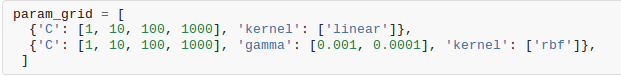
\includegraphics[width=\textwidth]{sklearn_material/grid}\\
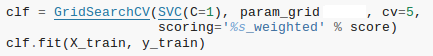
\includegraphics[width=.65\textwidth]{sklearn_material/grid_search}
\item Some estimators have path model, hence allow faster evaluation
  (e.g. LASSO).
\item Randomized techniques also exist, sometimes more efficient.
\item \textbf{Caveat:} Inner cross-validation loop $\neq$ outer
  cross-validation loop for parameter evaluation.
\end{itemize}
\end{frame}

\begin{frame}
\frametitle{Parameter setting and overfit} 

Using one cross-validation loop for learning parameters and evaluating
yields \textbf{optimistic bias} and \textbf{poor generalization}:
Overfit ! {\tiny \url{http://nilearn.github.io/building_blocks/estimator_choice.html}}

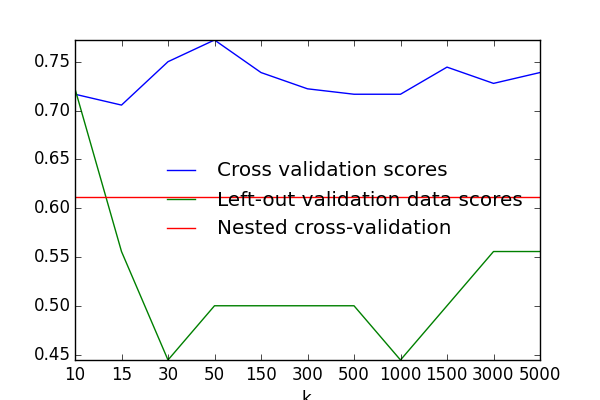
\includegraphics[width=.8\textwidth]{sklearn_material/plot_haxby_grid_search_11.png}

\end{frame}

    \subsection{Accuracy Measures}                                           
\begin{frame}
\frametitle{Accuracy measures for regression}
\begin{itemize}
\item {\bf Root-mean squared error} for point predictions.
\item {\bf Correlation coefficient} for point predictions.
\item {\bf Log predictive probability} can be used for probabilistic predictions.
\item {\bf Expected loss/risk} for point predictions for decision making.
\end{itemize}
\end{frame}

\begin{frame}
\frametitle{Accuracy measures for binary classification}
\begin{columns}
\column{0.7\textwidth}
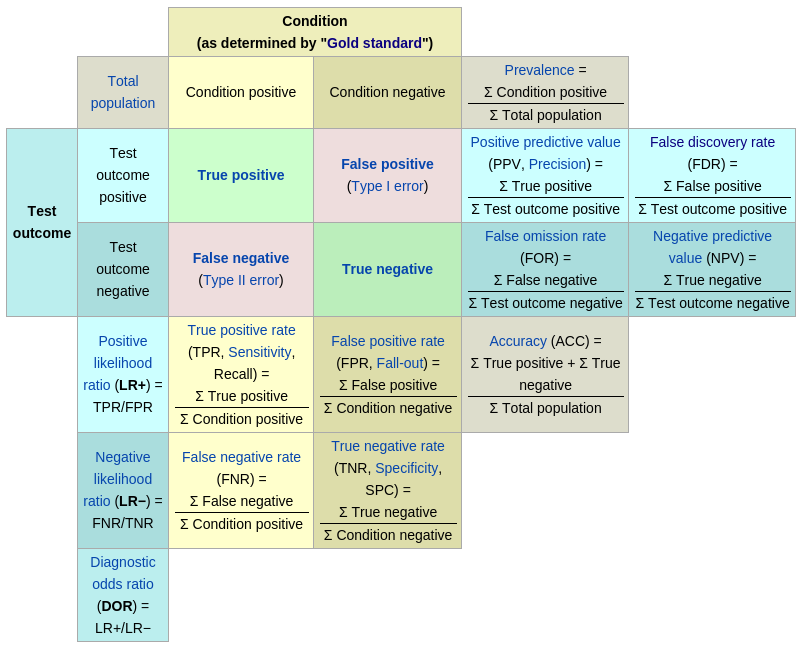
\includegraphics[width=\textwidth]{contingency_table_wikipedia}
%\vspace{0.25cm}
\column{0.3\textwidth}
%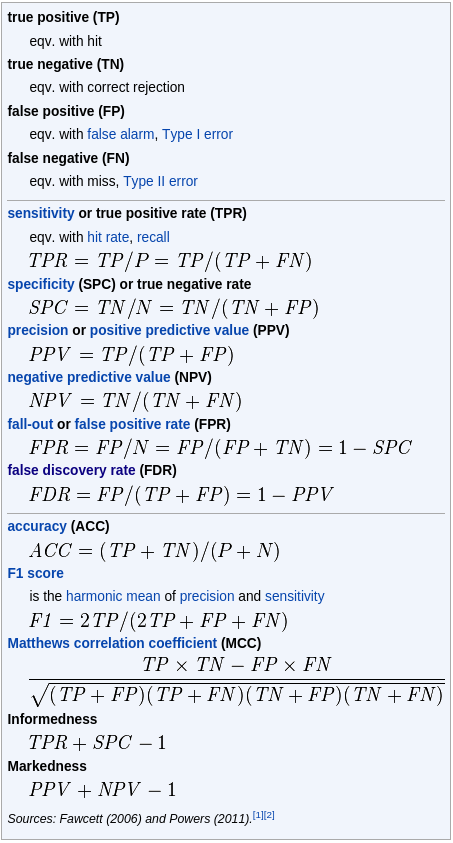
\includegraphics[width=\textwidth]{spec_sens_wikipedia}
\begin{tiny}
Wikipedia contributors, ``Sensitivity and specificity,'' Wikipedia, The Free Encyclopedia, \url{http://en.wikipedia.org/w/index.php?title=Sensitivity\_and\_specificity\&oldid=655245669} (accessed April 9, 2015).\par
\end{tiny}
\end{columns}
\end{frame}

\begin{frame}
\frametitle{Accuracy measures from ROC curve}
\begin{columns}
\column{0.5\textwidth}
The {\bf Receiver operating characteristic} (ROC) curve is a plot of \emph{true-positive rate} (sensitivity) versus \emph{false-positive rate} (1-specificity) over the full range of possible thresholds.\par
\vspace{0.25cm}
The {\bf area under the curve} (AUC) is the integral under the ROC curve.\par
\column{0.5\textwidth}
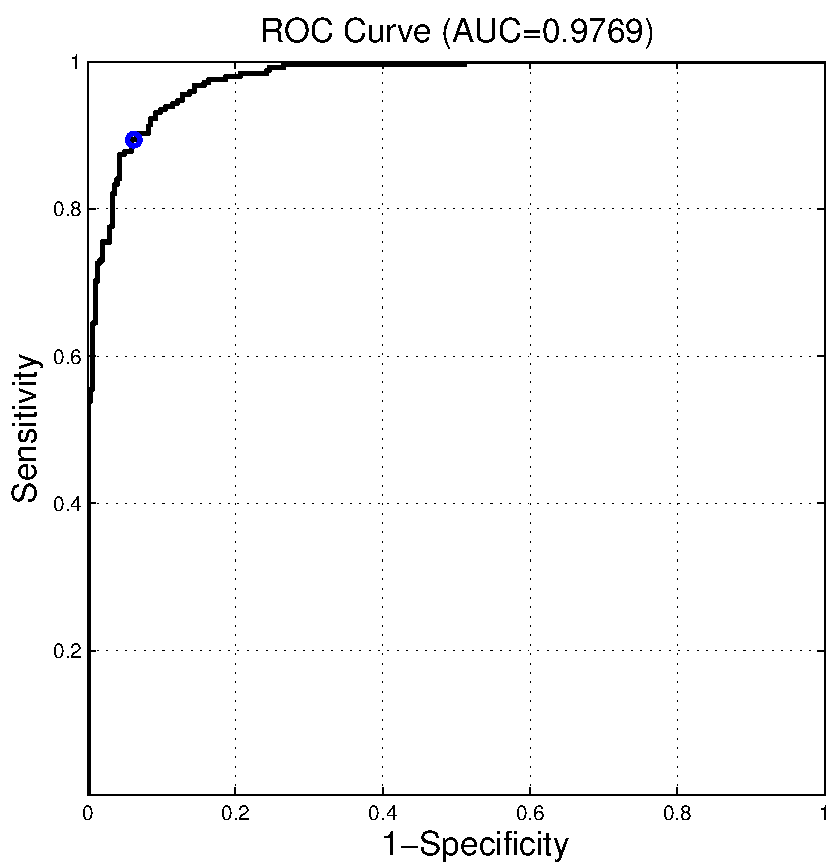
\includegraphics[width=\textwidth]{roc}
\end{columns}
\end{frame}

\begin{frame}
\frametitle{Log predictive probability}
Some data are more easily classified than others.\par
Probabilistic classifiers provide a level of confidence for each prediction.
\begin{align*}
p(y_*|{\bf x}_*,{\bf y},{\bf X},\theta)
\end{align*}
Quality of predictions can be assessed using the {\bf test log predictive probability}:
\begin{align*}
\tfrac{1}{m}\sum_{i=1}^m \log_2 p(y_{*i}\!=\!t_i|{\bf x}_{*i},{\bf y},{\bf X},\theta)
\end{align*}
After subtracting the baseline measure, this shows the average bits of information given by the model.\par
\vspace{0.25cm}
\begin{tiny}
Rasmussen \& Williams. ``Gaussian Processes for Machine Learning'', MIT Press (2006).\par
\url{http://www.gaussianprocess.org/gpml/}\par
\end{tiny}
\end{frame}


    \subsection{Parameter Tuning}                                            \include{ParameterTuning}
\section{Overview of the main methods}

\begin{frame}
\frametitle{Overview of classification tools}
\hspace*{-1cm}
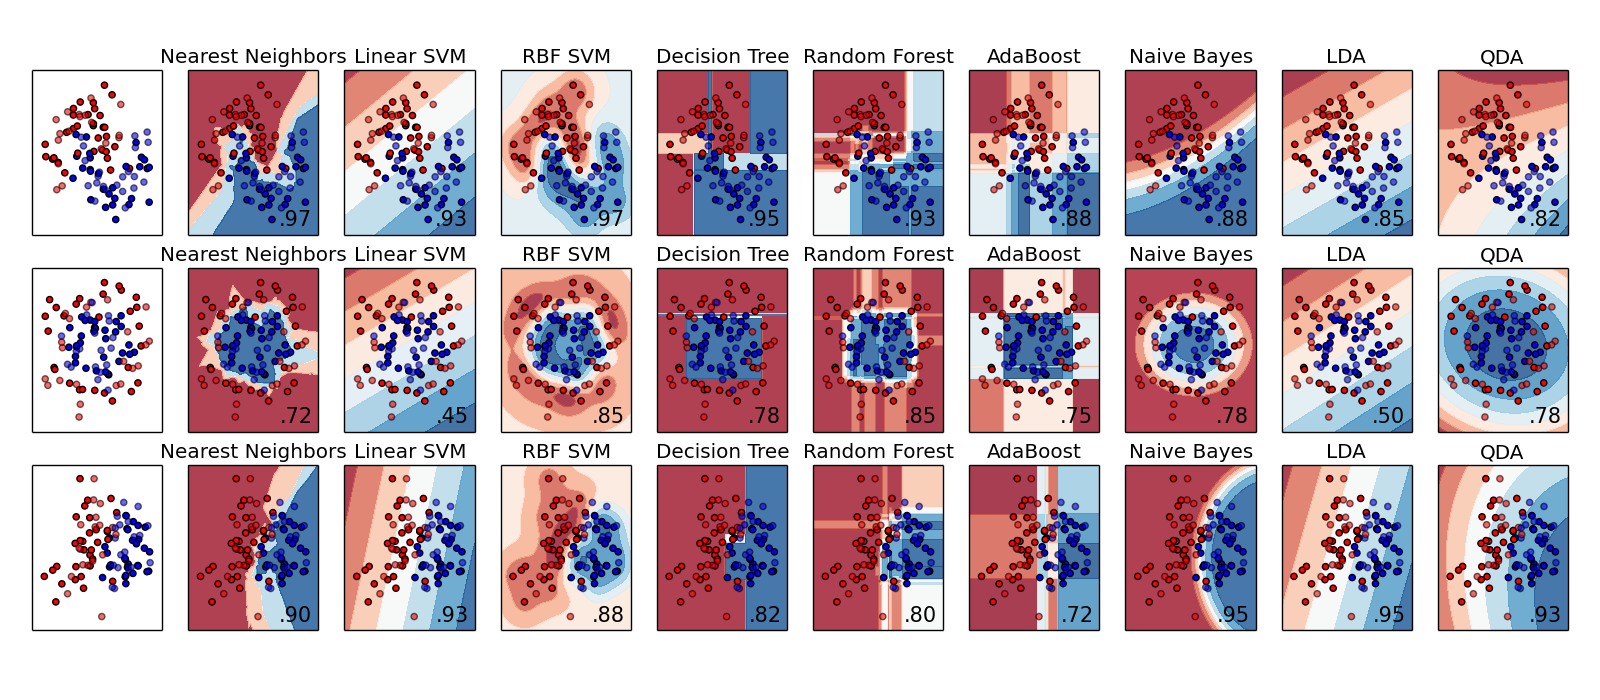
\includegraphics[width=1.2\textwidth]{sklearn_material/plot_classifier_comparison_001.png}\\
Only one rule: No tool wins in all situations. 
\end{frame}



    \subsection{Simple Generative Models: Naive Bayes, Linear Discriminant Analysis}       
\begin{frame}
\frametitle{Generative models for classification}
\begin{columns}[c]
\column{0.5\textwidth}
\begin{align*}
P(y\!=\!k|{\bf x}) = \frac{P(y\!=\!k) p({\bf x}|y\!=\!k)}{\sum_j P(y\!=\!j) p({\bf x}|y\!=\!j)}
\end{align*}
\column{0.5\textwidth}
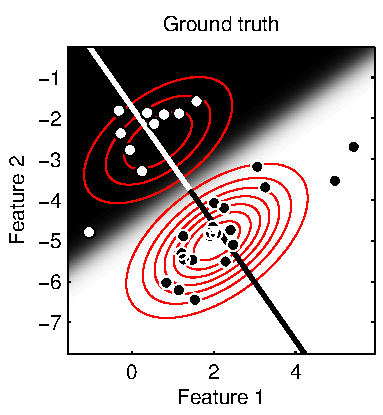
\includegraphics[width=\textwidth]{simple_ground_truth}
\end{columns}
\end{frame}

\begin{frame}
\frametitle{Linear discriminant analysis}
\begin{columns}[c]
\column{0.5\textwidth}
\begin{align*}
P(y\!=\!k|{\bf x}) = \frac{P(y\!=\!k) p({\bf x}|y\!=\!k)}{\sum_j P(y\!=\!j) p({\bf x}|y\!=\!j)}
\end{align*}
Assumes:
\begin{align*}
P({\bf x}|y\!=\!k) = \mathcal{N}({\bf x} | {\boldsymbol\mu}_k, \boldsymbol\Sigma)
\end{align*}
\column{0.5\textwidth}
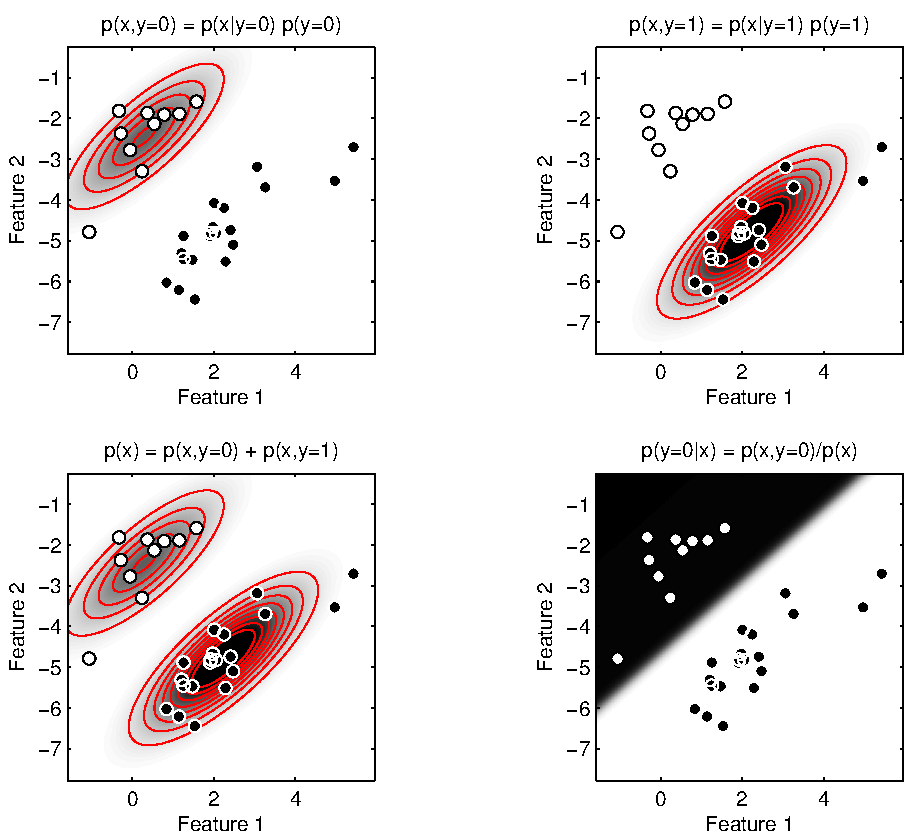
\includegraphics[width=\textwidth]{simple_fld}
\end{columns}
Model has $2p + p(p-1)$ parameters to estimate (two means and a single covariance).\par
Number of observations is $pn$ (size of inputs).
\end{frame}

\begin{frame}
\frametitle{Quadratic discriminant analysis}
\begin{columns}[c]
\column{0.5\textwidth}
\begin{align*}
P(y\!=\!k|{\bf x}) = \frac{P(y\!=\!k) p({\bf x}|y\!=\!k)}{\sum_j P(y\!=\!j) p({\bf x}|y\!=\!j)}
\end{align*}
Assumes different covariances:
\begin{align*}
P({\bf x}|y\!=\!k) = \mathcal{N}({\bf x} | {\boldsymbol\mu}_k, {\boldsymbol\Sigma}_k)
\end{align*}
\column{0.5\textwidth}
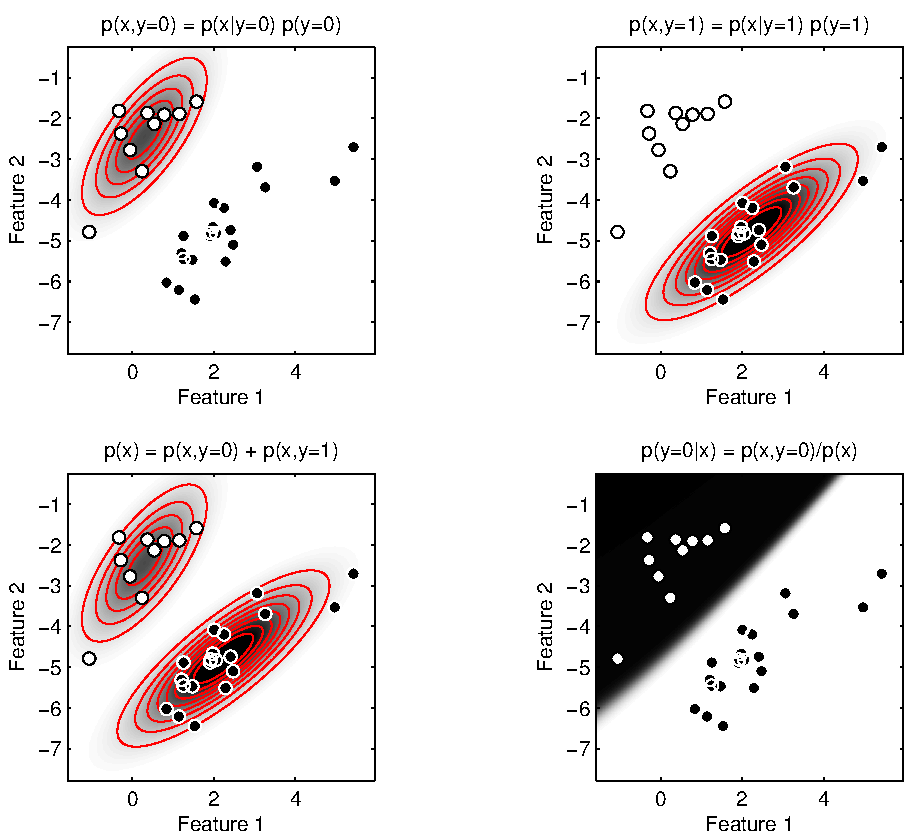
\includegraphics[width=\textwidth]{simple_qda}
\end{columns}
Model has $2p + 2p(p-1)$ parameters to estimate (two means and two covariances).\par
Number of observations is $pn$.
\end{frame}

\begin{frame}
\frametitle{Naive Bayes}
\begin{columns}[c]
\column{0.5\textwidth}
\begin{align*}
P(y\!=\!k|{\bf x}) = \frac{P(y\!=\!k) p({\bf x}|y\!=\!k)}{\sum_j P(y\!=\!j) p({\bf x}|y\!=\!j)}\cr
\end{align*}
Assumes that features are independent:
\begin{align*}
p({\bf x}|y\!=\!k) = \prod_i p(x_i|y\!=\!k)
\end{align*}
\column{0.5\textwidth}
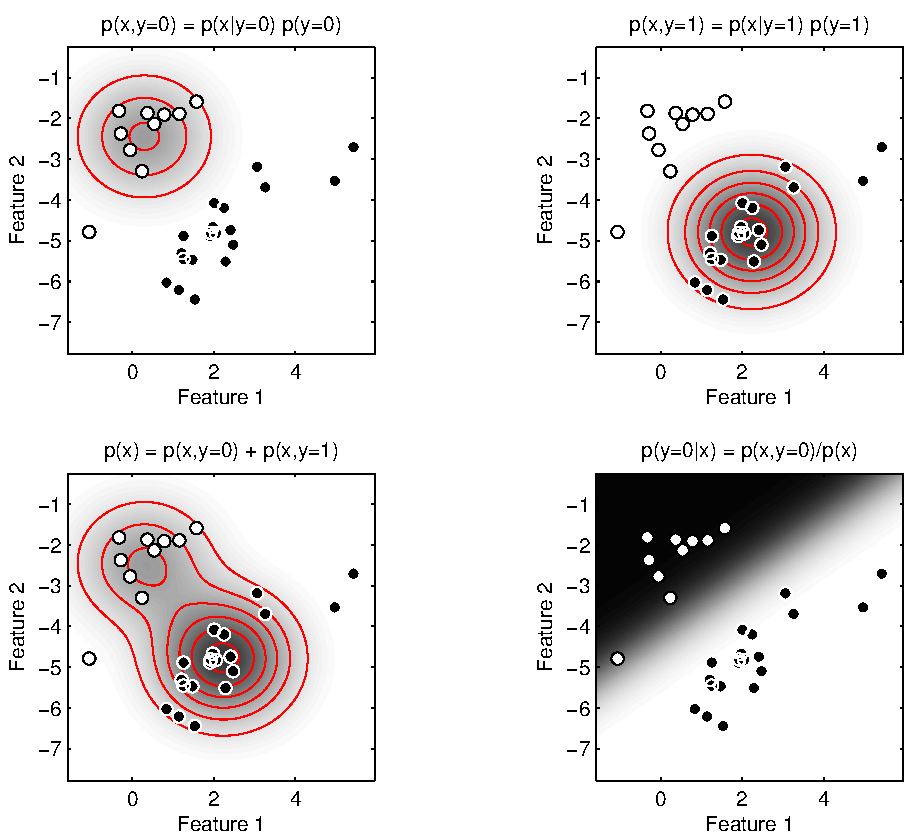
\includegraphics[width=\textwidth]{simple_naive_bayes}
\end{columns}
Model has variable number of parameters to estimate, but the above example has $3p$.\par
Number of observations is $pn$.
\end{frame}

\begin{frame}
\frametitle{Linear regression: maximum likelihood}
\begin{align*}
f({\bf x}_*) = {\bf a}^T {\bf x}_*
\end{align*}
Assuming Gaussian noise on ${\bf y}$, the ML estimate of ${\bf a}$ is by:
\begin{align*}
\hat{\bf a} = ({\bf X}{\bf X}^T)^{-1}{\bf X} {\bf y}
\end{align*}
where
\begin{align*}
{\bf X} = \begin{pmatrix}{\bf x}_1 & {\bf x}_2 & \hdots & {\bf x}_n\end{pmatrix}^T \text{, and }
{\bf y} = \begin{pmatrix}y_1 & y_2 & \hdots y_n\end{pmatrix}^T
\end{align*}
Model has $p$ parameters to estimate.\par
Number of observations is $n$ (number of targets).
\end{frame}

\begin{frame}
\frametitle{Linear regression: maximum posterior}
\begin{align*}
y \sim & \mathcal{N}({\bf a}^T {\bf x},\sigma^2)\\
{\bf a} \sim & \mathcal{N}({\bf 0},\Sigma_0)
\end{align*}
Maximum a posteriori (MAP) estimate of ${\bf a}$ is by:
\begin{align*}
\hat{\bf a} = \sigma^{-2}{\bf C}^{-1}{\bf X}{\bf y} \text{, where } {\bf C} = \sigma^{-2}{\bf X}{\bf X}^T + \Sigma_0^{-1}
\end{align*}
Number of estimated parameters and observations is ill defined.
\end{frame}

\begin{frame}
\frametitle{Linear regression: Bayesian}
\begin{align*}
p(y_* | {\bf x}_*, {\bf a}) = & \mathcal{N}({\bf a}^T{\bf x}_*, \sigma^2)\cr
p({\bf a}|{\bf y},{\bf X})  = & \mathcal{N}(\sigma^{-2}{\bf C}^{-1}{\bf X}{\bf y},{\bf C}^{-1}) \text{, where } {\bf C} = \sigma^{-2}{\bf X}{\bf X}^T + \Sigma_0^{-1}
\end{align*}
\begin{align*}
p(y_* | {\bf x}_*, {\bf y}, {\bf X}) = & \int_{\bf a} p(y_* | {\bf x}_*, {\bf a}) p({\bf a}|{\bf y},{\bf X}) d{\bf a}\cr
                                     = & \mathcal{N}(\sigma^{-2} {\bf x}_*^T {\bf C}^{-1} {\bf X} {\bf y}, {\bf x}_*^T{\bf C}^{-1}{\bf x}_*)
\end{align*}
Weights are integrated out - rather than estimated.\par
Estimated parameters may be $\sigma^2$, and parameters encoding $\Sigma_0$.
\end{frame}


\begin{frame}
\frametitle{Discriminative models for classification}
\begin{columns}[c]
\column{0.5\textwidth}
\begin{align*}
t = f({\bf a}^T {\bf x})
\end{align*}
where $f$ is some squashing function, eg:
\begin{itemize}
\item Heaviside step function.
\item Logistic function (inverse of Logit).
\item Normal CDF (inverse of Probit).
\end{itemize}
\column{0.5\textwidth}
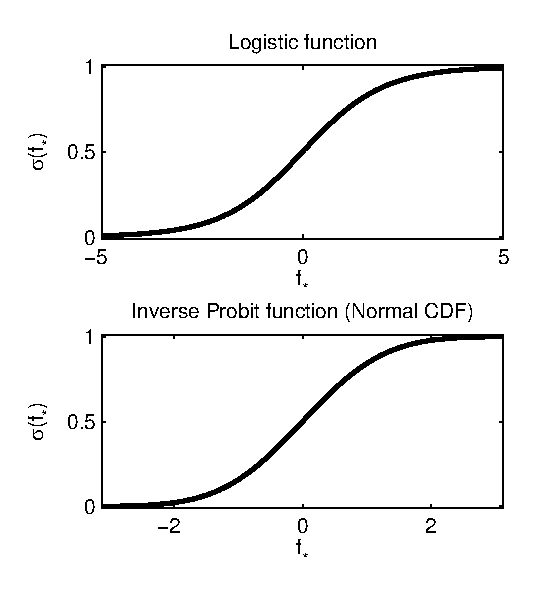
\includegraphics[width=.75\textwidth]{squashing}
\end{columns}
\end{frame}

\begin{frame}
\frametitle{Probabilistic classification}
\begin{columns}[c]
\column{0.5\textwidth}
\begin{align*}
P(y\!=\!k|{\bf x}) = \int_{\bf a} P(y\!=\!k|{\bf x},{\bf a}) p({\bf a}) d{\bf a}
\end{align*}
\column{0.5\textwidth}
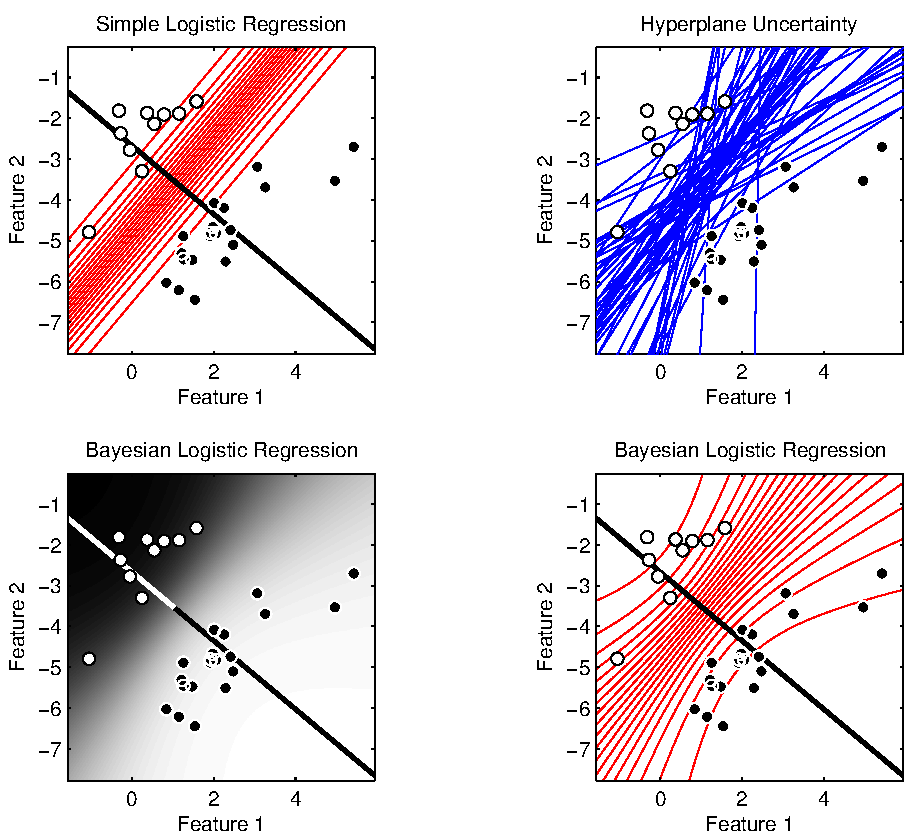
\includegraphics[width=\textwidth]{logistic_regr}
\end{columns}
\end{frame}

\begin{frame}
\frametitle{Woodbury matrix identity}
\begin{align*}
{\bf C}^{-1} = & \left(\sigma^{-2}{\bf X}{\bf X}^T + \Sigma_0^{-1}\right)^{-1}\\
             = & \Sigma_0 - \Sigma_0 {\bf X}({\bf I}\sigma^2 + {\bf X}^T \Sigma_0 {\bf X})^{-1} {\bf X} \Sigma_0
\end{align*}

\vspace{0.25cm}
\begin{tiny}
Wikipedia contributors, ``Woodbury matrix identity,'' Wikipedia, The Free Encyclopedia, \url{http://en.wikipedia.org/w/index.php?title=Woodbury\_matrix\_identity\&oldid=638370219} (accessed April 1, 2015).\par
\end{tiny}
\end{frame}


    \subsection{Simple Discriminative Models: Gaussian Processes, Support-Vector Machines} \begin{frame}
\frametitle{Linear regression: maximum likelihood}
A simple way to do regression is by:
\begin{align*}
f({\bf x}_*) = {\bf a}^T {\bf x}_*
\end{align*}
Assuming Gaussian noise on ${\bf y}$, the ML estimate of ${\bf a}$ is by:
\begin{align*}
\hat{\bf a} = ({\bf X}^T{\bf X})^{-1}{\bf X}^T {\bf y}
\end{align*}
where
\begin{align*}
{\bf X} = \begin{pmatrix}{\bf x}_1 & {\bf x}_2 & \hdots & {\bf x}_n\end{pmatrix}^T \text{, and }
{\bf y} = \begin{pmatrix}y_1 & y_2 & \hdots y_n\end{pmatrix}^T
\end{align*}
Model has $p$ parameters to estimate.\par
Number of observations is $n$ (number of targets).\par
Usualy needs dimensionality reduction, with (eg) SVD.
\end{frame}

\begin{frame}
\frametitle{Linear regression: maximum posterior}
We may have prior knowledge about various distributions:
\begin{align*}
p(y_* | {\bf x}_*, {\bf a}) = & \mathcal{N}({\bf a}^T{\bf x}_*, \sigma^2)\cr
p({\bf a}) = & \mathcal{N}({\bf 0},\boldsymbol\Sigma_0)\cr
\end{align*}
Therefore,
\begin{align*}
p({\bf a}|{\bf y},{\bf X})  = & \mathcal{N}(\sigma^{-2}{\bf B}^{-1}{\bf X}^T{\bf y},{\bf B}^{-1}) \text{, where } {\bf B} = \sigma^{-2}{\bf X}^T{\bf X} + \boldsymbol\Sigma_0^{-1}
\end{align*}

Maximum a posteriori (MAP) estimate of ${\bf a}$ is by:
\begin{align*}
\hat{\bf a} = \sigma^{-2}{\bf B}^{-1}{\bf X}^T{\bf y} \text{, where } {\bf B} = \sigma^{-2}{\bf X}^T{\bf X} + \boldsymbol\Sigma_0^{-1}
\end{align*}
\end{frame}

\begin{frame}
\frametitle{Linear regression: Bayesian}
We may have prior knowledge about various distributions:
\begin{align*}
p(y_* | {\bf x}_*, {\bf a}) = & \mathcal{N}({\bf a}^T{\bf x}_*, \sigma^2)\cr
p({\bf a}) = & \mathcal{N}({\bf 0},\boldsymbol\Sigma_0)\cr
\end{align*}
Therefore,
\begin{align*}
p({\bf a}|{\bf y},{\bf X})  = & \mathcal{N}(\sigma^{-2}{\bf B}^{-1}{\bf X}^T{\bf y},{\bf B}^{-1}) \text{, where } {\bf B} = \sigma^{-2}{\bf X}^T{\bf X} + \boldsymbol\Sigma_0^{-1}
\end{align*}
Predictions are made by integrating out the uncertainty of the weights, rather than estimating them:
\begin{align*}
p(y_* | {\bf x}_*, {\bf y}, {\bf X}) = & \int_{\bf a} p(y_* | {\bf x}_*, {\bf a}) p({\bf a}|{\bf y},{\bf X}) d{\bf a}\cr
                                     = & \mathcal{N}(\sigma^{-2} {\bf x}_*^T {\bf B}^{-1} {\bf X}^T {\bf y}, {\bf x}_*^T{\bf B}^{-1}{\bf x}_*)
\end{align*}
Estimated parameters may be $\sigma^2$, and parameters encoding $\boldsymbol\Sigma_0$.
\end{frame}

\begin{frame}
\frametitle{Kernel methods: Woodbury matrix identity}
\begin{align*}
{\bf B}^{-1} = & \left(\sigma^{-2}{\bf X}^T{\bf X} + \boldsymbol\Sigma_0^{-1}\right)^{-1}\\
             = & \boldsymbol\Sigma_0 - \boldsymbol\Sigma_0 {\bf X}^T({\bf I}\sigma^2 + {\bf X} \boldsymbol\Sigma_0 {\bf X}^T)^{-1} {\bf X} \boldsymbol\Sigma_0
\end{align*}

\vspace{0.25cm}
\begin{tiny}
Wikipedia contributors, ``Woodbury matrix identity,'' Wikipedia, The Free Encyclopedia, \url{http://en.wikipedia.org/w/index.php?title=Woodbury\_matrix\_identity\&oldid=638370219} (accessed April 1, 2015).\par
\end{tiny}
Dimensions of ${\bf X}^T{\bf X}$ are $p \times p$.\par
Dimensions of ${\bf X} \boldsymbol\Sigma_0 {\bf X}^T$ are $n \times n$.\par
\end{frame}

\begin{frame}
\frametitle{Kernel methods: Gaussian process regression}
The predicted distribution is:
\begin{align*}
p(y_*|{\bf x}_*,{\bf y},{\bf X}) = &\mathcal{N}({\bf k}^T{\bf C}^{-1} {\bf y},c - {\bf k}^T {\bf C}^{-1} {\bf k})
\end{align*}
where:
\begin{align*}
{\bf C} = & {\bf X} \boldsymbol\Sigma_0 {\bf X}^T + {\bf I}\sigma^2\\
{\bf k} = & {\bf X} \boldsymbol\Sigma_0 {\bf x}_*\\
c = & {\bf x}_*^T \boldsymbol\Sigma_0 {\bf x}_* + \sigma^2
\end{align*}
\end{frame}

\begin{frame}
\frametitle{Kernel methods: nonlinear methods}
%\begin{columns}[c]
%\column{0.5\textwidth}
Sometimes, we want alternatives to ${\bf C} = {\bf X} \boldsymbol\Sigma_0 {\bf X}^T + {\bf I}\sigma^2$.\par
Nonlinearity is achieved by replacing the matrix ${\bf K} = {\bf X} \boldsymbol\Sigma_0 {\bf X}^T$ with some function of the data that gives a positive definite matrix encoding similarities.\par
eg
\begin{align*}
k({\bf x}_i,{\bf x}_j) = \theta_1 + \theta_2 {\bf x}_i \cdot {\bf x_j} + \theta_3 \exp\left(-\frac{||{\bf x}_i - {\bf x_j}||^2}{2 \theta_4^2}\right)
\end{align*}

Hyper-parameters $\theta_1$ to $\theta_4$ can be optimised in a number of ways.\par
%\column{0.5\textwidth}
%Examples include:
%\begin{itemize}
%\item Linear: $k({\bf x}_i,{\bf x}_j) = {\bf x}_i \cdot {\bf x}_k$
%\item 
%\end{itemize}
%\includegraphics[width=.75\textwidth]{nonlinear_kernels}
%\end{columns}
\end{frame}

\begin{frame}
\frametitle{Kernel methods: nonlinear methods}
\begin{columns}[cc]
\column{0.6\textwidth}
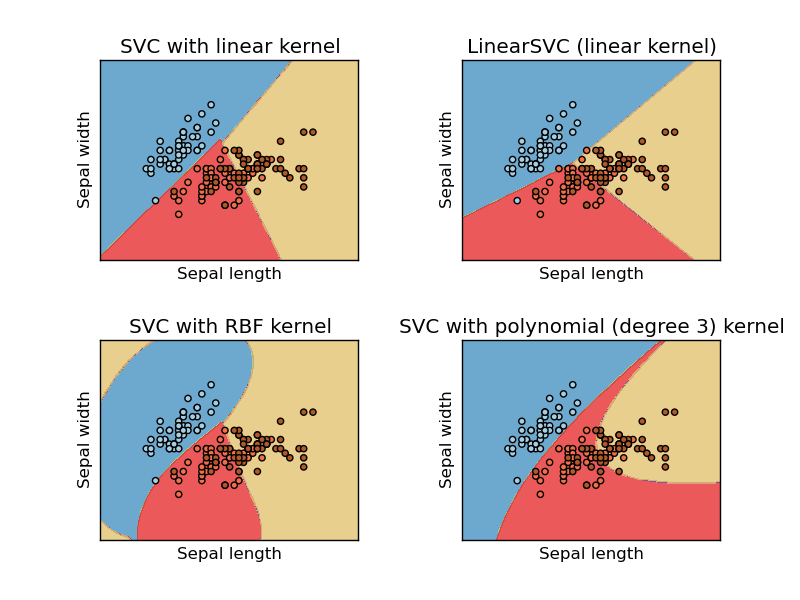
\includegraphics[width=\textwidth]{sklearn_material/plot_iris_0012.png}
\column{0.4\textwidth} Non-linear methods are useful in low-dimension
to adapt the shape of decision boundaries.
\end{columns}
For large $p$, small $n$ problems, nonlinear methods do not seem to help much.\par
Nonlinearity also reduces interpretability.
\end{frame}

\begin{frame}
\frametitle{Discriminative models for classification}
\begin{columns}[c]
\column{0.5\textwidth}
\begin{align*}
t = \sigma(f({\bf x}_*)) 
\end{align*}
where $\sigma$ is some squashing function, eg:
\begin{itemize}
\item Heaviside step function.
\item Logistic function (inverse of Logit).
\item Normal CDF (inverse of Probit).
\item Hinge loss (support vector machines)
\end{itemize}
\column{0.5\textwidth}
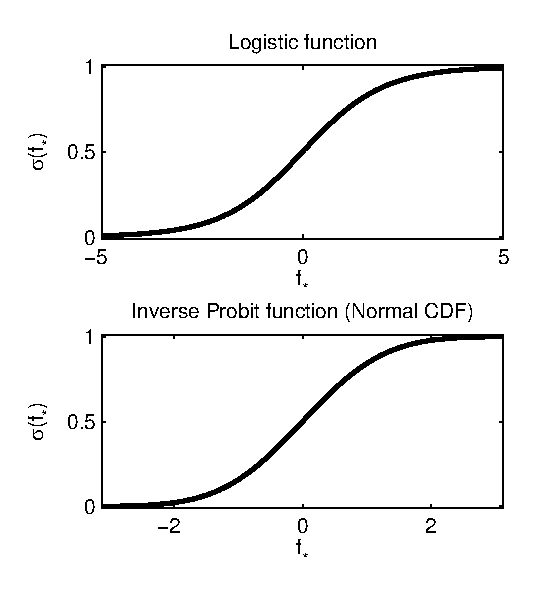
\includegraphics[width=.75\textwidth]{squashing}

\textbf{Bertrand: maybe a distinction should be introduced here between the decision function (typically the sign function) and the loss function used for training.}

\end{columns}
\end{frame}

\begin{frame}
\frametitle{Discriminative models for classification: convexity} 

In practice, the hinge and logistic losses yield a convex estimation
problem and are preferred.

\begin{align*}
\text{min}_{\mathbf{w}} \; \sum_{i=1}^n \mathcal{L}(y_i,\mathbf{X_i},\mathbf{w}) + \lambda \mathcal{R} (\mathbf{w})
\end{align*}


(M-estimators framework)
\begin{itemize}
\item $\mathcal{L}$ is the loss function (hinge, logistic, quadratic...)
\item $\mathcal{R}$ is the regularizer (typically a norm on $\mathbf{w}$) 
\item $\lambda > 0$ balances the two terms
\end{itemize}
$\mathcal{L}$ and $\mathcal{R}$ convex $\rightarrow$ unique minimizer (SVMs, $\ell_2$-logistic, $\ell_1$-logistic).

\end{frame}

\begin{frame}
\frametitle{Probabilistic classification}
\begin{columns}[c]
\column{0.5\textwidth}
Integrating over the uncertainty of the separating hyperplane allows probabilistic predictions further from the training data.\par
This is not usually done for methods such as the relevance-vector machine (RVM).\par
\vspace{0.25cm}
\begin{tiny}
Rasmussen, Carl Edward, and Joaquin Quinonero-Candela. ``Healing the relevance vector machine through augmentation.'' In Proceedings of the 22nd international conference on Machine learning, pp. 689-696. ACM, 2005.\par
\end{tiny}
\column{0.5\textwidth}
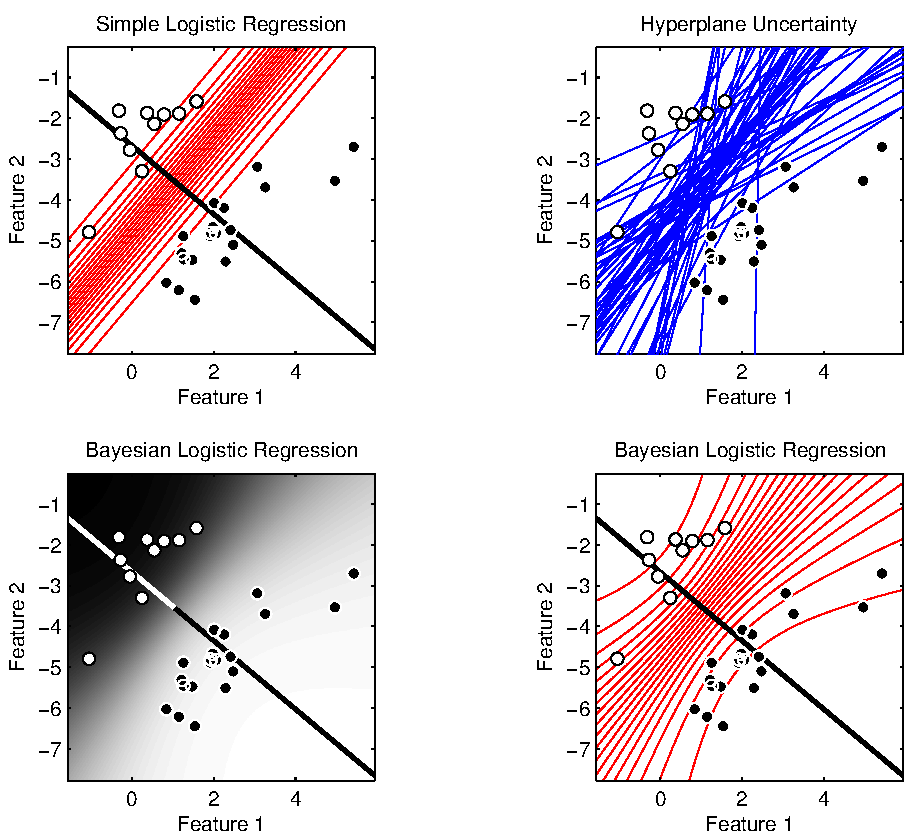
\includegraphics[width=\textwidth]{logistic_regr}
\end{columns}
\end{frame}

\begin{frame}
\frametitle{Probabilistic classification}
Making probabilistic predictions involves:
\begin{enumerate}
\item Computing the distribution of a latent variable corresponding to the test data (cf regression):
\begin{align*}
p(f_* | {\bf x}_*, {\bf y}, {\bf X}) = & \int_{\bf f} p(f_* | {\bf x}_*, {\bf f}) p({\bf f}|{\bf y},{\bf X}) d{\bf f}
\end{align*}
\item Using this distribution to give a probabilistic prediction:
\begin{align*}
P(y_*=1|{\bf x}_*,{\bf y},{\bf X}) = \int_{f_*} \sigma(f_*) p(f_*|{\bf x}_*,{\bf y},{\bf X}) df_*
\end{align*}
\end{enumerate}
Unfortunately, the second integral is analytically intractable, so approximations are needed.\par
\end{frame}

\begin{frame}
\frametitle{Probabilistic classification}
Approximate methods for probabilistic classification include:
\begin{itemize}
\item {\bf The Laplace Approximation} (LA).  Fastest, but less accurate.
\item {\bf Expectation Propagation} (EP).  More accurate than the Laplace approximation, but slightly slower.
\item {\bf MCMC} methods. The ``gold standard'', but very slow to draw lots of random samples.
\end{itemize}
\vspace{0.25cm}
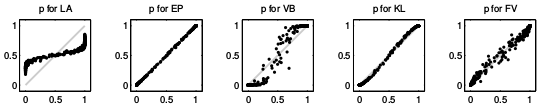
\includegraphics[width=\textwidth]{nickisch_figure}
\begin{tiny}
Nickisch, Hannes, and Carl Edward Rasmussen. ``Approximations for Binary Gaussian Process Classification.'' Journal of Machine Learning Research 9 (2008): 2035-2078.\par
\end{tiny}
\end{frame}

\begin{frame}
\frametitle{Support vector classification}
\begin{columns}[c]
\column{0.5\textwidth}
If you are only interested in binary predictions, support-vector machines are reasonably fast and accurate.\par
%Targets are ${\bf t} \in \{-1,1\}$.\\
%Solves a quadratic programming problem
%\begin{align*}
%\hat{\boldsymbol\alpha} = \argmin_{\boldsymbol\alpha} \tfrac{1}{2} {\boldsymbol\alpha}^T {\bf H}{\boldsymbol\alpha} - \sum_{i=1}^n \alpha_i,\\
%\text{subject to }
%{\bf t}^T{\boldsymbol\alpha} = 0 \text{ and }
%0 \le \alpha_i \le C\\
%\text{where }
%{\bf H} = \diag({\bf t}) {\bf X}{\bf X}^T \diag({\bf t})
%\end{align*}
%Binary prediction is by:
%\begin{align*}
%t_* = sgn(\sum_{i=1}^N t_i \alpha_i {\bf x}_i {\bf x}_*^T + b)
%\end{align*}
%where $b$ is a bias term.
\column{0.5\textwidth}
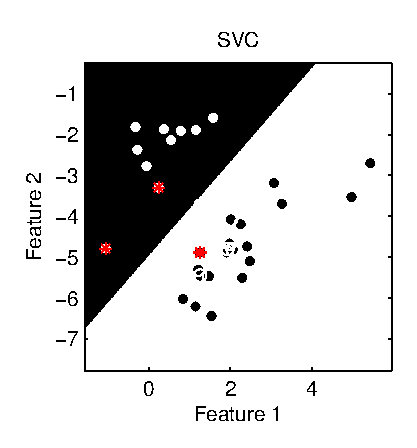
\includegraphics[width=\textwidth]{svc}
\end{columns}
\end{frame}


    \subsection{Basic Regularization Methods}                                \include{BasicRegularisationMethods}
\section{Model Averaging}
    \subsection{Boosting \& Bagging}                                         \begin{frame}
\frametitle{Ensemble learning}
Combining predictions from weak learners.
\begin{itemize}
\item {\bf Bootstrap aggregating (bagging)}
\begin{itemize}
\item Train several weak classifiers, with different models or randomly drawn subsets of the data.
\item Average their predictions with equal weight.
\end{itemize}
\item {\bf Boosting}
\begin{itemize}
\item A family of approaches, where models are weighted according to their accuracy.
\item AdaBoost is popular, but has problems with target noise.
\end{itemize}
\item {\bf Bayesian model averaging}
\begin{itemize}
\item Really a model selection method.
\item Relatively ineffective for combining models.
\end{itemize}
\item {\bf Bayesian model combination}
\begin{itemize}
\item Shows promise.
\end{itemize}
\end{itemize}
\begin{tiny}
Monteith, et al. ``Turning Bayesian model averaging into Bayesian model combination.'' Neural Networks (IJCNN), The 2011 International Joint Conference on. IEEE, 2011.\par
\end{tiny}
\end{frame}

%\begin{frame}
%\frametitle{Random Forests}
%\end{frame}

\begin{frame}
\frametitle{Boosting}

Reduce sequentially the bias of the combined
estimator. \\

Examples: AdaBoost, Gradient Tree Boosting, ...\\

\begin{center}
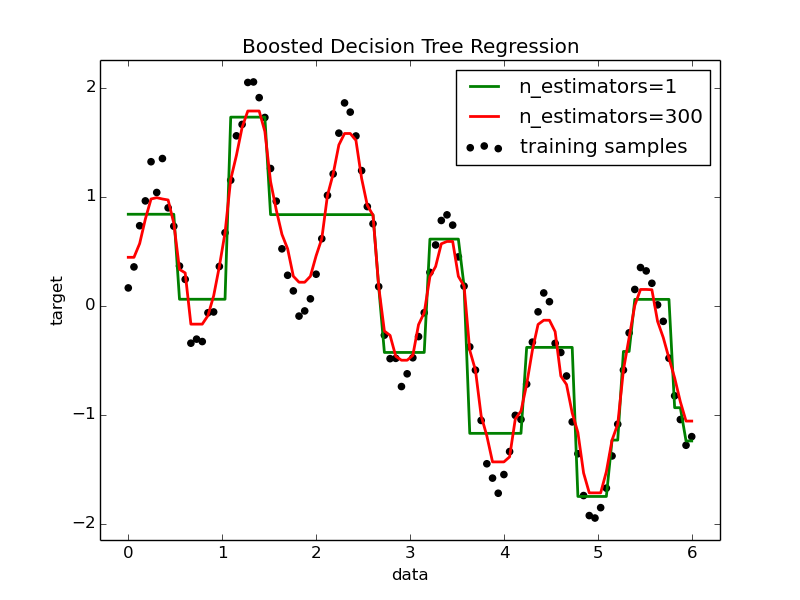
\includegraphics[width=.75\linewidth]{sklearn_material/plot_adaboost_regression.png}
\end{center}

\end{frame}


\begin{frame}
\frametitle{Bagging}

Build several estimators independently and average their
predictions. Reduce the variance.\\

Examples: Bagging methods, Forests of randomized trees, ...\\

\begin{center}
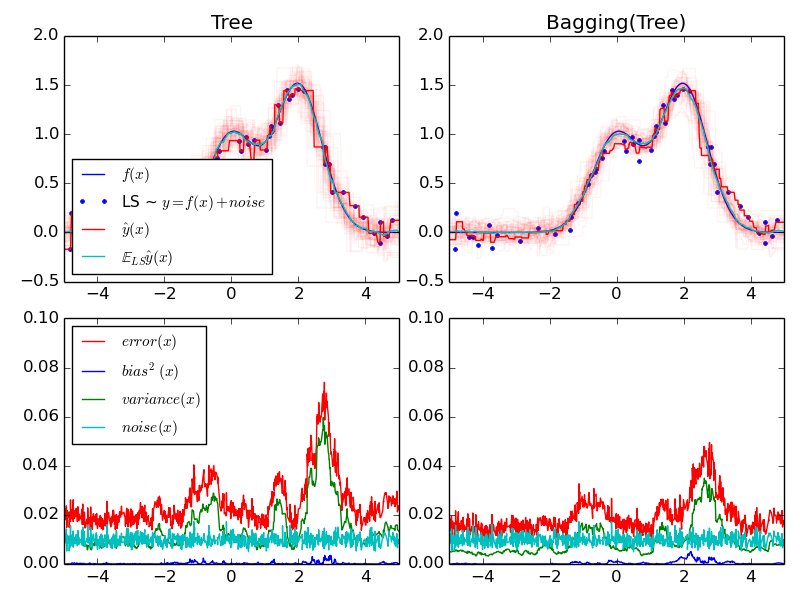
\includegraphics[width=.7\linewidth]{sklearn_material/bias_variance.png}
\end{center}

\end{frame}



\begin{comment}
\begin{frame}
\frametitle{Ensemble learning}
ensemble methods: combine the predictions of several
base estimators (generalizability / robustness)  

\begin{itemize}
\item 
\textbf{averaging methods:} build several
estimators independently and average their predictions. Recuce the variance:\\

Examples: Bagging methods, Forests of randomized trees, ...
\item
\textnf{boosting methods:} reduce sequentially the bias of the combined
estimator. \\

Examples: AdaBoost, Gradient Tree Boosting, ...
\end{itemize}
\end{frame}
\end{comment}



    \subsection{Decision trees and Random Forests}                           \include{RandomForests}
    \subsection{Tools: scikit-learn, pronto, nilearn, pymvpa}                \include{Tools}
\end{document}

